% ─────────────────────────────────────────────────────────────
\section{Matériel et protocole applicatif}

\subsection{Format des messages CAN}

Le protocole utilise le format standard \textbf{CAN~2.0A}, avec un
identifiant sur 11~bits. Cet identifiant est découpé en deux parties :

\begin{table}[H]
\centering
\begin{tabular}{|c|c|c|}
\hline
Bits & Rôle & Valeurs \\
\hline
b10 -- b7 & Type de message & 0000 = pas d'analogique, 0001 = analogique \\
\hline
b6 -- b0 & Adresse de la carte (7 bits) & DIP2--DIP7, avec inversion du DIP1 \\
\hline
\end{tabular}
\caption{Découpage de l'identifiant CAN sur 11 bits}
\end{table}

\subsection{Configuration par DIP-switch}

Les 8 interrupteurs du DIP-switch ont la fonction suivante :

\begin{table}[H]
\centering
\begin{tabular}{|c|p{11cm}|}
\hline
\textbf{DIP 1} & Bit de poids faible de l'adresse pour les messages
reçus. Son inverse est utilisé pour les messages émis.
Seul ce bit diffère entre deux cartes jumelées. \\
\hline
\textbf{DIP 2--7} & 6 bits de poids supérieur de l'adresse (DIP7~=~MSB). \\
\hline
\textbf{DIP 8} & Active (1) ou désactive (0) l'émission / la réception des
messages analogiques. Les messages tout-ou-rien sont toujours traités. \\
\hline
\end{tabular}
\caption{Affectation des 8 interrupteurs DIP}
\end{table}


\newpage
\section{Mesures sur bus libre à 1~Mbps}

Les premières mesures sont réalisées avec une seule paire de cartes A1/A2 et
une vitesse de bus de \num{1}~Mbps.

\paragraph{Remarque importante.}
Lors des premières mesures, la condition empêchant l'envoi d'un message
inchangé n'était pas encore implémentée. Le bus était donc occupé en continu
par des messages tout-ou-rien, ce qui n'a pas empêché les premières
observations, mais a probablement influencé les mesures de latence et de
gigue. Faute de temps, ces mesures n'ont pas pu être refaites. Le problème a
été corrigé avant les mesures sur bus chargé à \num{200}~kbps (section~\ref{section5}).

\subsection{Analyse d'une trame CAN}

Pour cette mesure, le DIP8 est mis à 0 (pas de trafic analogique). L'entrée
tout-ou-rien n°0 est basculée pour provoquer l'émission d'un unique message.
La figure~\ref{fig:trame} montre la trame CAN capturée à l'oscilloscope sur la
ligne \texttt{CANH}. On y distingue les différents champs caractéristiques
d'une trame CAN 2.0A : \textbf{SOF} (1 bit dominant), \textbf{champ
d'arbitration} (11 bits d'identifiant + RTR), \textbf{champ de contrôle}
(IDE, r0, DLC), \textbf{champ de données}, \textbf{CRC} (15
bits + délimiteur), \textbf{ACK} (slot + délimiteur) et enfin \textbf{EOF}.

\begin{figure}[H]
    \centering
    \begin{tikzpicture}
        \node[anchor=south west,inner sep=0] (img)
            {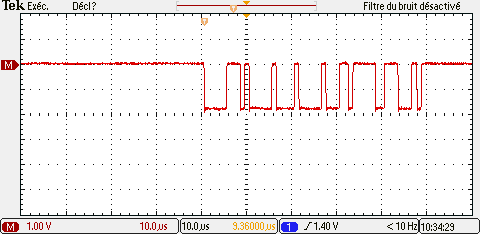
\includegraphics[width=0.95\textwidth]{images/TEK00001.PNG}};
        \begin{scope}[x={(img.south east)},y={(img.north west)}]
            % Field x-boundaries (normalized 0..1 along image width)
            \def\xSOFs{0.425}   % SOF start
            \def\xSOFe{0.437}   % SOF end (1 bit ~ 5 px)
            \def\xArbE{0.555}   % end of arbitration (ID + RTR), ~13 bits
            \def\xCtrlE{0.620}  % end of control (IDE+r0+DLC), ~6-7 bits
            \def\xDataE{0.700}  % end of data (8-9 bits)
            \def\xCRCE{0.860}   % end of CRC (15+1 delim)
            \def\xACKE{0.890}   % end of ACK (slot + delim, 2 bits)
            \def\xEOFE{0.965}   % end of EOF (7 bits, recessive)
            % Bar above image (bbox extended via invisible nodes)
            \def\ybar{1.06}
            \def\ylab{1.10}
            % Vertical dashed separators down onto the trace area
            \foreach \x in {\xSOFs, \xSOFe, \xArbE, \xCtrlE, \xDataE, \xCRCE, \xACKE, \xEOFE} {
                \draw[blue!70, dashed, thin] (\x, 0.20) -- (\x, \ybar);
            }
            % Horizontal bar across the whole frame
            \draw[blue!70, thick] (\xSOFs, \ybar) -- (\xEOFE, \ybar);
            % Labels above bar
            \node[blue!70!black, font=\scriptsize, anchor=south, rotate=40]
                at (\xSOFs, \ylab) {SOF};
            \node[blue!70!black, font=\scriptsize, anchor=south]
                at ({(\xSOFe+\xArbE)/2}, \ylab) {Arbitration};
            \node[blue!70!black, font=\scriptsize, anchor=south]
                at ({(\xArbE+\xCtrlE)/2}, \ylab) {Ctrl};
            \node[blue!70!black, font=\scriptsize, anchor=south]
                at ({(\xCtrlE+\xDataE)/2}, \ylab) {Data};
            \node[blue!70!black, font=\scriptsize, anchor=south]
                at ({(\xDataE+\xCRCE)/2}, \ylab) {CRC};
            \node[blue!70!black, font=\scriptsize, anchor=south, rotate=40]
                at ({(\xCRCE+\xACKE)/2}, \ylab) {ACK};
            \node[blue!70!black, font=\scriptsize, anchor=south]
                at ({(\xACKE+\xEOFE)/2}, \ylab) {EOF};
            % Force bbox extension so labels are not clipped
            \path (0, 1.18);
        \end{scope}
    \end{tikzpicture}
    \caption{Trame CAN complète capturée sur \texttt{CANH} à \num{1}~Mbps
    (base de temps 10~µs/div). Les champs ont été repérés a posteriori}
    en s'appuyant sur la durée d'un bit ($\approx$~1~µs) et la structure
    standard CAN~2.0A.
    \label{fig:trame}
\end{figure}

La figure~\ref{fig:bit} permet de vérifier la durée d'un bit à l'aide des
curseurs de l'oscilloscope : $\Delta x = 1{,}000$~µs entre deux fronts
correspondant à un bit, soit une fréquence de bit de
$f_{\text{bit}} = 1{,}00$~MHz ou \num{1}~Mbps.

\begin{figure}[H]
    \centering
    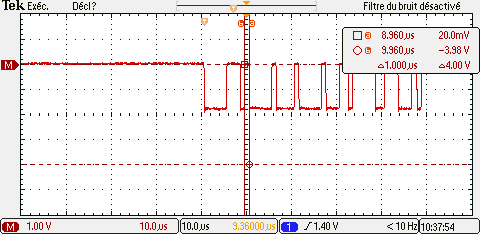
\includegraphics[width=0.75\textwidth]{images/TEK00002.PNG}
    \caption{Mesure de la durée d'un bit : $\Delta x = 1{,}00$~µs
    $\Rightarrow$ \num{1}~Mbps.}
    \label{fig:bit}
\end{figure}

\subsection{Comportement en cas de problème de transmission}

Le câble CAN est débranché, puis l'émission d'un message est provoquée. On
observe sur la figure~\ref{fig:debranche} une activité continue sur la
ligne du côté émetteur : le MCP2515 n'obtient jamais d'ACK du receveur et
retransmet indéfiniment le même message. La LED rouge s'allume
brièvement à chaque erreur de transmission.

\begin{figure}[H]
    \centering
    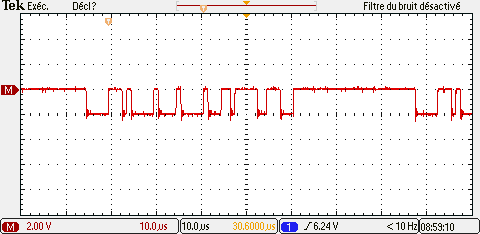
\includegraphics[width=0.75\textwidth]{images/TEK00003.PNG}
    \caption{Signal du côté émetteur, câble CAN débranché.}
    \label{fig:debranche}
\end{figure}


\subsection{Latence et gigue à vide}
\label{sec:latence_vide}

Un signal carré à \num{25}~Hz est injecté sur une entrée tout-ou-rien de la
carte~A1, et le signal récupéré sur la sortie correspondante de la carte~A2
est observé simultanément à l'oscilloscope. La latence mesurée est le
décalage entre le front d'entrée et le front de sortie.

\begin{table}[H]
\centering
\begin{tabular}{|l|c|}
\hline
Grandeur & Valeur mesurée \\
\hline
Latence minimale $t_{\min}$ & $416$~µs \\
\hline
Latence maximale $t_{\max}$ & $1{,}05$~ms \\
\hline
Gigue $J = t_{\max} - t_{\min}$ & $\approx 632$~µs \\
\hline
\end{tabular}
\caption{Latence et gigue à \num{1}~Mbps, bus sans trafic.}
\label{tab:latence_vide}
\end{table}

\begin{figure}[H]
    \centering
    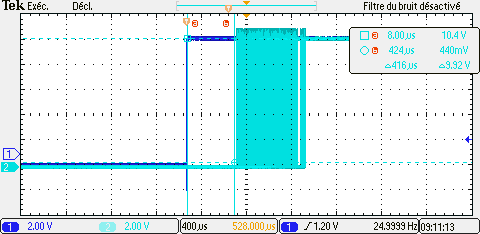
\includegraphics[width=0.75\textwidth]{images/TEK00005.PNG}
    \caption{Latence minimale $t_{\min} = 416$~µs (curseurs de l'oscilloscope).}
\end{figure}

\begin{figure}[H]
    \centering
    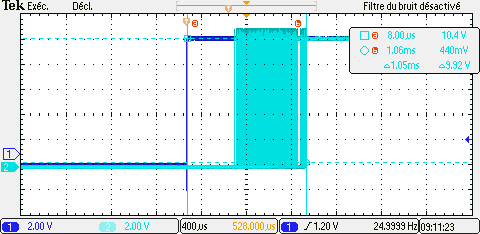
\includegraphics[width=0.75\textwidth]{images/TEK00006.PNG}
    \caption{Latence maximale $t_{\max} = 1{,}05$~ms.}
\end{figure}

\begin{figure}[H]
    \centering
    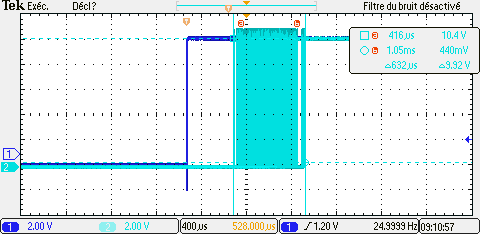
\includegraphics[width=0.75\textwidth]{images/TEK00004.PNG}
    \caption{Superposition en persistance infinie mettant en évidence la
    gigue $\Delta t \approx 632$~µs.}
\end{figure}

\subsection{Transmission des valeurs analogiques (trafic spontané)}

Le DIP8 de la carte A1 est mis à 1 pour activer l'émission des messages
analogiques, tandis que l'entrée analogique est laissée à un potentiel fixe.
La figure~\ref{fig:trafic} montre pourtant un trafic continu sur le
bus.

\begin{figure}[H]
    \centering
    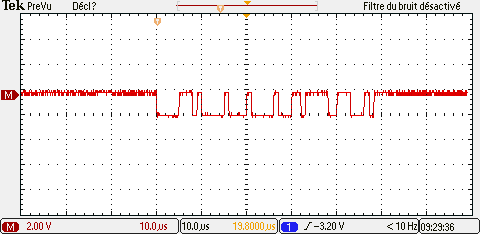
\includegraphics[width=0.75\textwidth]{images/TEK00007.PNG}
    \caption{Trafic observé avec l'entrée analogique laissée fixe.}
    \label{fig:trafic}
\end{figure}

\paragraph{Explication.}
Bien que l'entrée soit branchée sur un potentiel fixe, le bruit électronique
du CAN de l'Arduino Mega fait varier la valeur lue à chaque itération.
Comme notre critère d'émission est « envoyer si la valeur a
changé depuis le dernier message », un message est généré quasiment à chaque
tour de boucle.

\subsection{Transmission d'un signal sinusoïdal}

Un signal sinusoïdal est injecté sur l'entrée analogique AIN0 de la carte~A1
et le signal est observé simultanément en entrée (A1) et en sortie analogique
(AOUT0 de la carte~A2).

\paragraph{Intervalle entre messages.}
La figure~\ref{fig:intervalle} met en évidence, en zoomant sur les marches
d'escalier de la sortie, l'intervalle temporel entre deux messages
analogiques reçus : $\Delta t \approx 1{,}10$~ms.
\begin{quote}
\footnotesize
\noindent\textbf{Note.} L'image est globalement correcte, mais un problème
lors de l'acquisition a légèrement décalé les curseurs ; la valeur de
$\Delta t$ mesurée reste cependant juste.
\end{quote}

\begin{figure}[H]
    \centering
    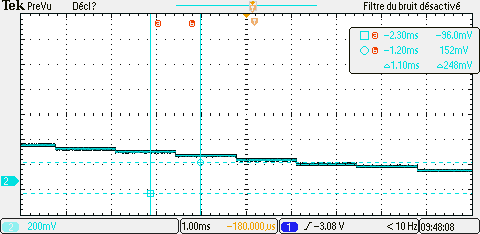
\includegraphics[width=0.75\textwidth]{images/TEK00008.PNG}
    \caption{Intervalle entre deux mises à jour successives de la sortie
    analogique : \num{1{,}10}~ms.}
    \label{fig:intervalle}
\end{figure}

\paragraph{Qualité à basse fréquence (6~Hz).}
Pour $f = 6$~Hz, la sortie analogique reproduit fidèlement l'entrée
sinusoïdale (figure~\ref{fig:sin6}). L'escalier n'est pas visible à cette
échelle temporelle, la période étant très grande devant l'intervalle de
\num{1{,}1}~ms entre messages.

\begin{figure}[H]
    \centering
    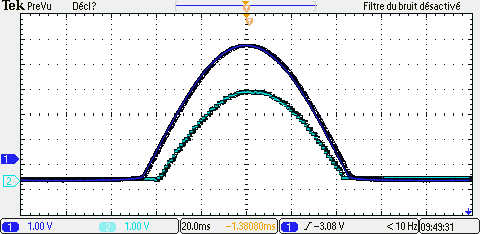
\includegraphics[width=0.75\textwidth]{images/TEK00009.PNG}
    \caption{Signaux d'entrée (bleu) et de sortie (turquoise) à $f = 6$~Hz.}
    \label{fig:sin6}
\end{figure}

\Needspace{0.45\textheight}
\paragraph{Qualité à plus haute fréquence (30~Hz).}
Pour $f = 30$~Hz (figure~\ref{fig:sin30}), la sortie présente de nettes
marches d'escalier. 

\begin{figure}[H]
    \centering
    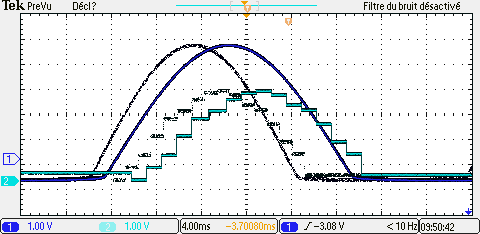
\includegraphics[width=0.75\textwidth]{images/TEK00010.PNG}
    \caption{Signaux d'entrée (bleu) et de sortie (turquoise) à $f = 30$~Hz.
    La sortie est visiblement dégradée et retardée.}
    \label{fig:sin30}
\end{figure}

\paragraph{Influence de la fréquence.}
La qualité de reproduction est directement liée au nombre d'échantillons
par période du signal sinusoïdal. L'intervalle entre messages étant fixe
($\approx$~1,1~ms), la dégradation devient perceptible dès que la période du
signal se rapproche de cette durée, typiquement au-delà de quelques dizaines
de hertz.

% ─────────────────────────────────────────────────────────────
\newpage
\section{Mesures sur bus chargé à 200~kbps}
\label{section5}
Pour cette partie, deux paires de cartes (A1/A2 et B1/B2) partagent le même
bus CAN, la vitesse est réduite à \num{200}~kbps et les adresses sont fixées
comme suit :

\begin{table}[H]
\centering
\begin{tabular}{|c|c|}
\hline
Carte & Adresse (DIP1 $\rightarrow$ DIP7) \\
\hline
A1 & 22 (0110 100) \\
A2 & 23 (1110 100) \\
B1 & 72 (0001 001) \\
B2 & 73 (1001 001) \\
\hline
\end{tabular}
\caption{Adresses configurées pour les mesures à 4 cartes.}
\end{table}

\subsection{Latence et gigue sous charge}

Un signal carré à \num{500}~Hz est injecté sur une entrée tout-ou-rien de A1
et la sortie correspondante est observée sur A2. Dans un premier temps, seul
le couple A1/A2 est actif, puis le même signal est ajouté sur B1 afin
d'introduire du trafic supplémentaire.

\begin{table}[H]
\centering
\begin{tabular}{|l|c|c|c|}
\hline
Configuration & $t_{\min}$ & $t_{\max}$ & Gigue $J$ \\
\hline
Couple A1/A2 seul (sans trafic) & $604$~µs & $800$~µs & $\approx 192$~µs \\
\hline
A1/A2 + trafic sur B1/B2        & $604$~µs & $1{,}07$~ms & $\approx 468$~µs \\
\hline
\end{tabular}
\caption{Latence et gigue à \num{200}~kbps avec et sans trafic concurrent.}
\label{tab:latence_charge}
\end{table}

\begin{figure}[H]
    \centering
    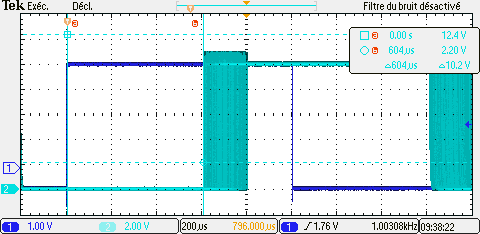
\includegraphics[width=0.75\textwidth]{images/TEK00011.PNG}
    \caption{Latence minimale A1$\rightarrow$A2, bus libre : $604$~µs.}
\end{figure}

\begin{figure}[H]
    \centering
    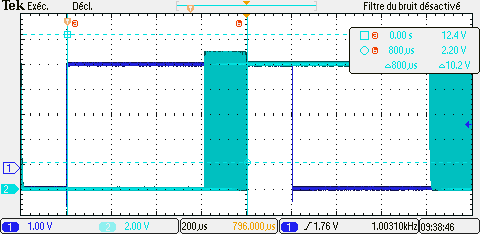
\includegraphics[width=0.75\textwidth]{images/TEK00012.PNG}
    \caption{Latence maximale A1$\rightarrow$A2, bus libre : $800$~µs.}
\end{figure}

\begin{figure}[H]
    \centering
    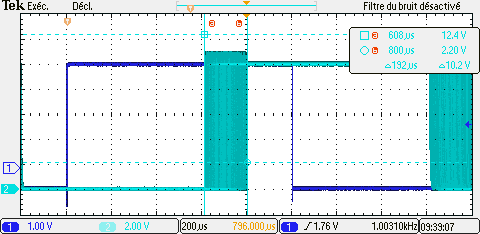
\includegraphics[width=0.75\textwidth]{images/TEK00013.PNG}
    \caption{Gigue A1$\rightarrow$A2 bus libre : $\Delta t \approx 192$~µs.}
\end{figure}

\begin{figure}[H]
    \centering
    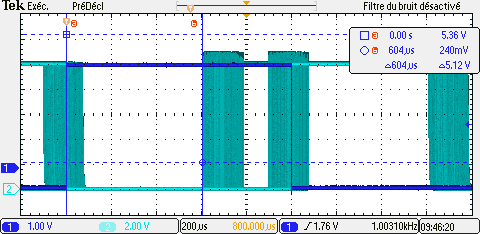
\includegraphics[width=0.75\textwidth]{images/TEK00014.PNG}
    \caption{Latence minimale A1$\rightarrow$A2 avec trafic B1/B2 : $604$~µs.}
\end{figure}

\begin{figure}[H]
    \centering
    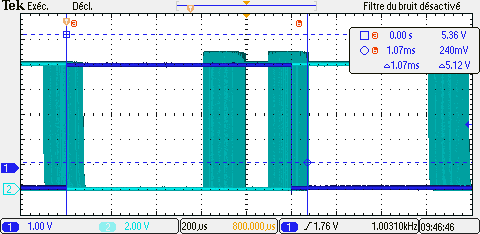
\includegraphics[width=0.75\textwidth]{images/TEK00015.PNG}
    \caption{Latence maximale A1$\rightarrow$A2 avec trafic B1/B2 :
    $1{,}07$~ms.}
\end{figure}

\begin{figure}[H]
    \centering
    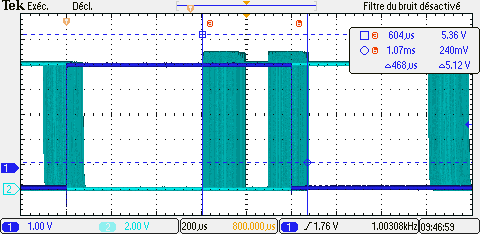
\includegraphics[width=0.75\textwidth]{images/TEK00016.PNG}
    \caption{Gigue A1$\rightarrow$A2 avec trafic B1/B2 :
    $\Delta t \approx 468$~µs.}
\end{figure}

\paragraph{Interprétation.}
\begin{itemize}
    \item La latence minimale reste constante (\num{604}~µs) : quand
    le bus est libre au moment de l'émission, la durée d'envoi d'un message
    est indépendante du trafic potentiel.
    \item En revanche, la latence maximale augmente (\num{800}~µs
    $\rightarrow$ \num{1{,}07}~ms) car le message d'A1 doit parfois
    attendre la fin d'un message concurrent B1$\rightarrow$B2 avant
    d'accéder au bus, conformément au mécanisme d'arbitration non destructive
    du protocole CAN.
    \item La gigue augmente donc fortement ($\approx 192$~µs
    $\rightarrow$ $\approx 468$~µs), directement dépendante de la durée
    d'un message concurrent (\num{\approx 550}~µs à \num{200}~kbps).
\end{itemize}

\subsection{Transmission d'un signal sinusoïdal sur bus chargé}

Un signal sinusoïdal à \num{50}~Hz est utilisé dans cette partie ; le bus
étant à \num{200}~kbps, l'intervalle entre messages analogiques est plus grand
qu'à \num{1}~Mbps, ce qui se traduit par des marches d'escalier déjà bien
visibles sur la sortie.

\paragraph{Étape 1 — B2 $\rightarrow$ B1 seul.}
Seul ce flux analogique circule. Le signal est reproduit avec marches
d'escalier mais sans retard ni instabilité apparente
(figure~\ref{fig:sin_b2b1}).

\begin{figure}[H]
    \centering
    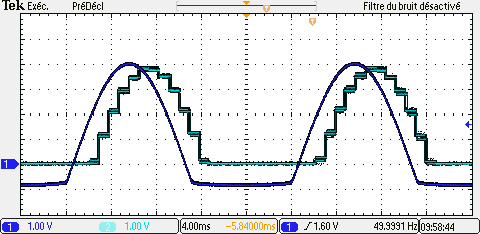
\includegraphics[width=0.75\textwidth]{images/TEK00020.PNG}
    \caption{Sinusoïde 50~Hz B2$\rightarrow$B1 seul
    (base~4~ms/div).}
    \label{fig:sin_b2b1}
\end{figure}

\paragraph{Étape 2 — ajout de B1 $\rightarrow$ B2.}
On active la sinusoïde dans le sens opposé. Le signal précédent devient
moins stable (il « bouge » davantage sur l'écran de l'oscilloscope) :
chaque message doit désormais partager le bus avec le flux inverse, ce qui
introduit une gigue supplémentaire dans l'arrivée des échantillons
(figure~\ref{fig:sin_b1b2}).

\begin{figure}[H]
    \centering
    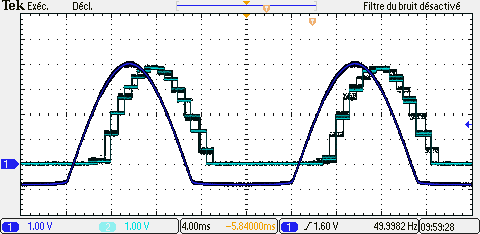
\includegraphics[width=0.75\textwidth]{images/TEK00021.PNG}
    \caption{Ajout du flux B1$\rightarrow$B2 : la sortie devient moins
    stable.}
    \label{fig:sin_b1b2}
\end{figure}

\Needspace{0.45\textheight}

\paragraph{Étape 3 — ajout de A2 $\rightarrow$ A1.}
Un troisième flux analogique est activé entre les cartes A. La sortie
observée se dégrade encore, avec une amplitude réduite et des marches plus
grossières (figure~\ref{fig:sin_a2a1}).

\begin{figure}[H]
    \centering
    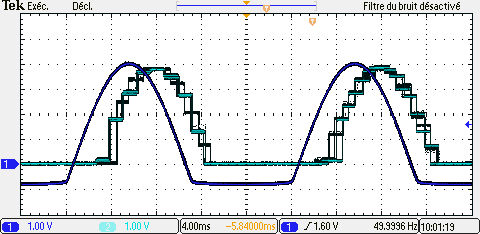
\includegraphics[width=0.75\textwidth]{images/TEK00022.PNG}
    \caption{Ajout du flux A2$\rightarrow$A1 : dégradation supplémentaire.}
    \label{fig:sin_a2a1}
\end{figure}

\paragraph{Étape 4 — ajout de A1 $\rightarrow$ A2.}
Avec les quatre flux analogiques actifs simultanément, le bus est saturé :
la sortie observée est trop en retard, ne suit quasiment plus la
consigne et reste à la valeur basse.§
(figure~\ref{fig:sin_a1a2}).

\begin{figure}[H]
    \centering
    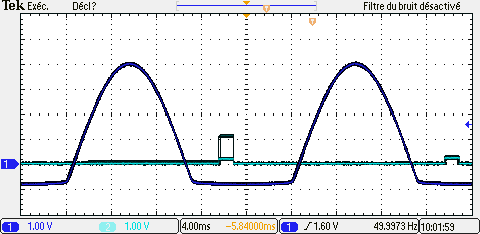
\includegraphics[width=0.75\textwidth]{images/TEK00023.PNG}
    \caption{Les 4 flux actifs : le bus est saturé, la sortie est en retard
    et ne reproduit plus correctement la sinusoïde.}
    \label{fig:sin_a1a2}
\end{figure}

\paragraph{Bilan.}
Chaque ajout d'un flux analogique (sinusoïde~50~Hz) augmente la charge du
bus. Tant que la charge reste modérée, l'arbitration CAN absorbe les
collisions et les signaux restent reproduits. Une fois le bus proche de la
saturation, l'intervalle entre messages analogiques reçus devient supérieur
à la période du signal à transmettre, et la qualité de reproduction
s'effondre.
